\section{Mapping low-loss EELS in polytypic WS$_2$}
\label{sec:results_sample}

Following the discussion of the vacuum ZLP analysis, we now
present the application of our machine learning strategy to parametrise the ZLP
arising in spectra recorded on specimens, specifically for
EELS measurements acquired in different regions
of the WS$_2$ nanoflowers presented in Sect.~\ref{sec:tmd}.
%
The resulting ZLP parametrisation will be applied to isolate the inelastic
contribution in each spectrum.
%
We will use these subtracted spectra first to determine the bandgap type and energy 
value from the behaviour of the onset region and second to identify excitonic
transitions at very low energy losses.

In this section we begin by presenting the training dataset, composed by two groups of EEL spectra recorded
in thick and thin regions of the WS$_2$  nanoflowers respectively.
%
Then we discuss the subtraction procedure, the choice of hyper-parameters, and the error propagation
to the physical predictions.
%
The resulting subtracted spectra provide the information
required to extract the value and type of the bandgap
and to characterise excitonic transitions for different regions of these polytypic WS$_2$ nanostructures.

\subsection{Training dataset}

Low-magnification TEM images  and the corresponding
spectral images of two representative regions of
the WS$_2$ nanoflowers, denoted as sample A and B  respectively, are displayed in Fig.~\ref{fig:ws2positions}.
%
These spectral images have been recorded in the regions marked by a green square
in the associated TEM images, and contain an individual EEL spectrum in each pixel.
%
We indicate the specific locations where
EEL spectra have been recorded, including the in-vacuum measurements acquired
for calibration purposes.
%
Note that in sample B  the differences in contrast are related to the material
thickness, with higher contrast corresponding to thinner regions.

These two samples are characterised by rather different structural morphologies.
%
While sample A is composed
by a relatively thick region of WS$_2$, sample B corresponds to a region where thin petals
overlap between them.
%
In other words, sample A is composed by bulk WS$_2$ while in sample B some specific regions
could be rather thinner, down to the few monolayers level.
%
This thickness information has been be determined
by means of the {\tt Digital~Micrograph}  software.

%%%%%%%%%%%%%%%%%%%%%%%%%%%%%%%%%%%%%%%%%%%%%%%%%%%%%%%%%%%%%%%%%%%%%%%
\begin{figure}[t]
\begin{centering}
  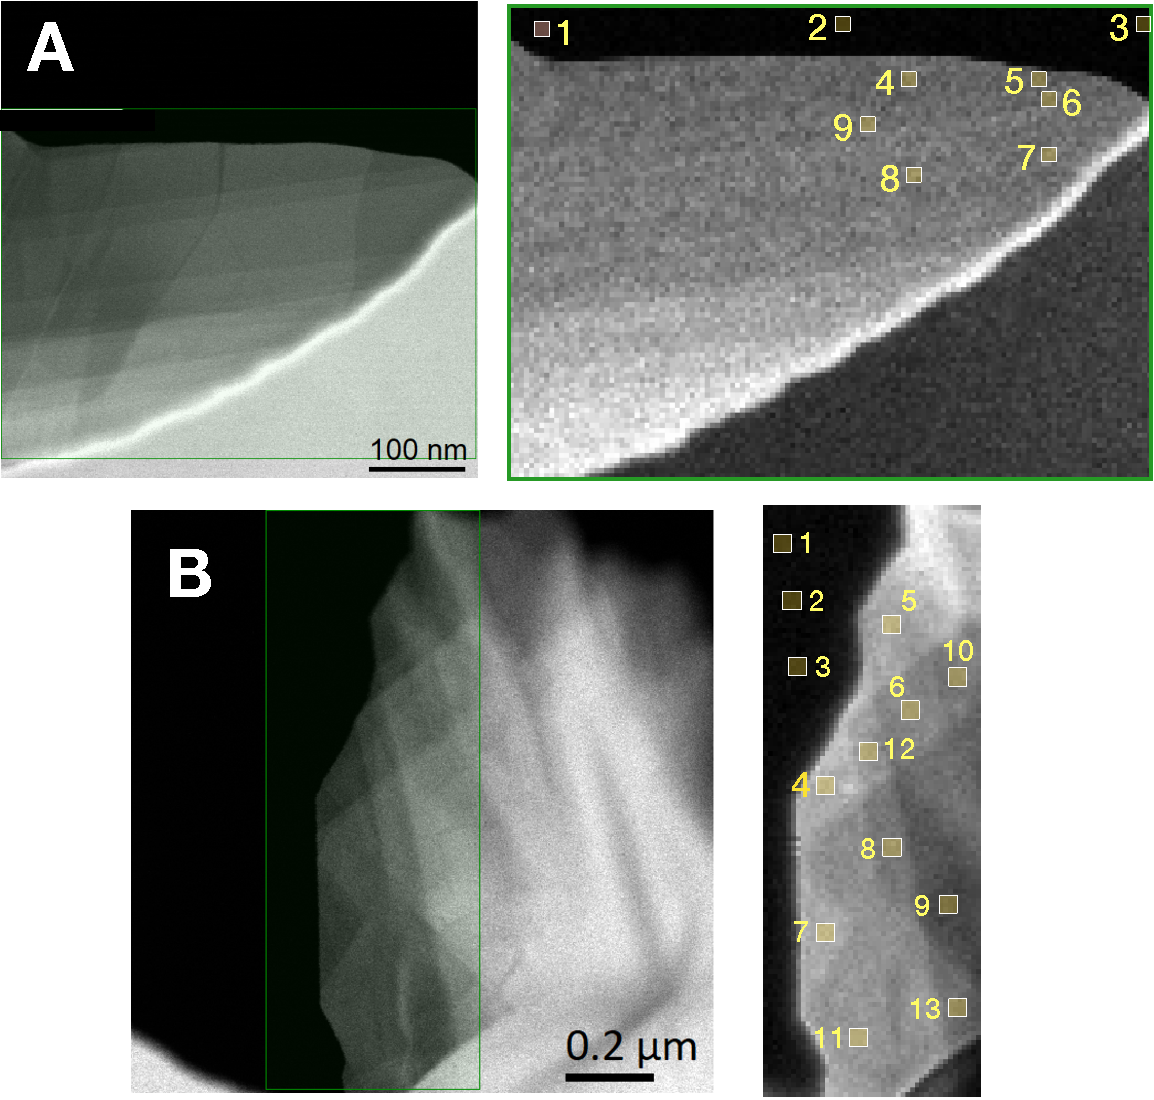
\includegraphics[width=0.92\linewidth]{plots/Spectra_location.pdf}
  \caption{Low-magnification TEM images (left) and the corresponding
    spectral images (right panels) of two different regions of
    the WS$_2$ nanoflowers, denoted as sample A (upper) and sample B (lower panels) respectively.
    %
    The spectral images have been recorded in the regions marked by a green square
    in the associated TEM images, and contain an individual EEL spectrum in each pixel.
    %
    We indicate the locations where representative
    EEL spectra have been selected. 
    %
    In the left panel of sample B, the difference in contrast is correlated to the material
    thickness, with higher contrast indicating thinner regions of the nanostructure.
    %
    The morphological differences between the two samples are discussed in the text.
  }
\label{fig:ws2positions}
\end{centering}
\end{figure}
%%%%%%%%%%%%%%%%%%%%%%%%%%%%%%%%%%%%%%%%%%%%%%%%%%%%%%%%%%%%%%%%%%%%%%%%%%

One of the main goals of this study is demonstrating that our ZLP-subtraction method exhibits
a satisfactory performance for spectra taken with different microscopes and operation conditions.
%
With this motivation, the EELS measurements acquired on specimens A and B have
been obtained varying both the microscopes and their settings.
%
Specifically, the TEM and EELS measurements acquired in specimen A  are based on a JEOL 2100F
microscope with a cold field-emission
gun and equipped with an aberration corrector,
operated at 60 kV and where a Gatan GIF Quantum was used for
the EELS analysis.
%
The corresponding measurements on specimen B  were recorded instead
using a JEM ARM200F monochromated microscope operated at 60 kV and equipped with a GIF quantum ERS.
%
See Methods for more details.

In Table~\ref{table:sampledata} we collect the most relevant properties of the spectra collected
in the locations indicated in Fig.~\ref{fig:ws2positions} using the same format as
in Table~\ref{table:vacuumdata}.
%
As we just mentioned, the spectra from samples A and B
have been acquired with different microscopes and thus features of the ZLP
such as the FWHM are expected to be different.
%
From this table one can observe how the ZLP for the spectra acquired on sample A exhibit
a FWHM about five times larger as compared to those of sample B.
%
This difference in energy resolution can be understood from the fact that the EELS spectra from sample B, unlike those
from sample A, were recorded with a TEM equipped with monochromator.

%%%%%%%%%%%%%%%%%%%%%%%%%%%%%%%%%%%%%%%%%%%%%%%%%%%%%%%%%%%%%%%%%%%%%%%%%%%%%%%%%%%%%%%%%%%%%
%%%%%%%%%%%%%%%%%%%%%%%%%%%%%%%%%%%%%%%%%%%%%%%%%%%%%%%%%%%%%%%%%%%%%%%%%%%%%%%%%%%%%%%%%%%%%
\begin{table}[t]
  \begin{center}
            \renewcommand{\arraystretch}{1.50}
  \begin{tabular}{@{}ccccccccc}
\br
Set & $t_{\rm exp}$ {(}ms{)} & $E_{\rm b}$ {(}keV{)} & $N_{\rm sp}$ & $N_{\rm dat}$ & $\Delta E_{\rm min}$~(eV)  & $\Delta E_{\rm max}$~(eV)  & FWHM~(meV)  \\ 
\mr
A        &       1       &        60         &   6      &    1918    &     -4.1       & 45.5 & $ 470\pm 10 $  \\
B        &       190       &        60       &   10     &    2000    &     -0.9        & 9.1   & $ 87 \pm 5$ \\
\br
  \end{tabular}
    \end{center}
  \caption{\small Same as Table~\ref{table:vacuumdata} for the EEL spectra taken on specimens A and B.
    %
    The location on the WS$_2$ nanoflowers where each spectra has been recorded
    is indicated in Fig.~\ref{fig:ws2positions}.
  }
   \label{table:sampledata}
\end{table}
%%%%%%%%%%%%%%%%%%%%%%%%%%%%%%%%%%%%%%%%%%%%%%%%%%%%%%%%%%%%%%%%%%%%%%%%%%%%%%%%%%%%%%%%%%%%%%%%%5
%%%%%%%%%%%%%%%%%%%%%%%%%%%%%%%%%%%%%%%%%%%%%%%%%%%%%%%%%%%%%%%%%%%%%%%%%%%%%%%%%%%%%%%%%%%%%

In the following we will present results for representative spectra
corresponding to specific choices of the locations indicated in Fig.~\ref{fig:ws2positions}.
%
The full set of recorded spectra is available  within {\tt EELSfitter},
the code used to produce the results of this analysis, and
whose installation
and usage instructions are summarised in Appendix~\ref{sec:installation}.

\subsection{Subtraction procedure}

In Table~\ref{table:sampledata_summary} we collect
the mean value and uncertainty of the first local minimum, $\Delta E|_{\rm min}$.
averaged over the spectra corresponding to samples A and B from
Fig.~\ref{fig:ws2positions}.
%
The location of the first minimum is relatively stable
among all the spectra belonging to a given set.
%
This indicates that the onset of the inelastic contributions $I_{\rm inel}$ does
not change significantly as we move between different regions of the sample.
%
We also indicate there
the corresponding values of the hyper-parameters
$\Delta E_{\rm I}$ and $\Delta E_{\rm II}$ defined in Fig.~\ref{fig:EELS_toy}.
%
Recall that only
the data points with $\Delta E \le \Delta E_{\rm I}$ are used for the training
of the neural network model.
%
The model training is performed for a range of $\Delta E_{\rm I}$ values,
subject to the condition that $\Delta E_{\rm I} \le \Delta E_{\rm min}$, to validate
the stability of the results.
%
The optimal value of $\Delta E_{\rm I}$ is determined by the condition
that Eq.~(\ref{eq:rder}) satisfies $\mathcal{R}^{(j)}_{\rm der}(\Delta E)\simeq 0.9$, indicating
that the shape of the intensity profile for the sample spectra differs by more than 10\%
as compared to their vacuum counterparts.

%%%%%%%%%%%%%%%%%%%%%%%%%%%%%%%%%%%%%%%%%%%%%%%%%%%%%%%%%%%%%%%%%%%%%%%%%%%%%%%%%%%%%%%%%%%%%
%%%%%%%%%%%%%%%%%%%%%%%%%%%%%%%%%%%%%%%%%%%%%%%%%%%%%%%%%%%%%%%%%%%%%%%%%%%%%%%%%%%%%%%%%%%%%
\begin{table}[t]
  \begin{center}
            \renewcommand{\arraystretch}{1.50}
  \begin{tabular}{@{}ccccccccc}
\br
Set & $\Delta E|_{\rm min}$~(eV)  &  $\Delta E_{\rm I}$~(eV)  &  $\Delta E_{\rm II}$~(eV)   \\
\mr
A        &    $2.70\pm0.06$               &          1.8        &      12         \\
B        &    $1.80\pm0.04$               &          1.4        &      6        \\
\br
  \end{tabular}
    \end{center}
  \caption{\small The mean value and uncertainty of the first local minima, $\Delta E|_{\rm min}$,
    averaged over the spectra corresponding to samples A and B from
    Fig.~\ref{fig:ws2positions}.
    %
    We also indicate
     the corresponding values of the hyper-parameters
     $\Delta E_{\rm I}$ and $\Delta E_{\rm II}$ defined in Fig.~\ref{fig:EELS_toy} used for the training
     of the neural network model.
    %
  }
   \label{table:sampledata_summary}
\end{table}
%%%%%%%%%%%%%%%%%%%%%%%%%%%%%%%%%%%%%%%%%%%%%%%%%%%%%%%%%%%%%%%%%%%%%%%%%%%%%%%%%%%%%%%%%%%%%%%%%5
%%%%%%%%%%%%%%%%%%%%%%%%%%%%%%%%%%%%%%%%%%%%%%%%%%%%%%%%%%%%%%%%%%%%%%%%%%%%%%%%%%%%%%%%%%%%%

In the region $\Delta E \ge \Delta E_{\rm II}$, the training set includes only the pseudo-data
that implements the $I_{\rm ZLP}(\Delta E)\to 0$ constraint.
 %
The values for $\Delta E_{\rm II}$ were determined from the spectra recorded in vacuum
following the same procedure as explained 
in Sect.~\ref{sec:results_vacuum}, based on requiring $\mathcal{R}_{\rm sig}(\Delta E_{\rm II})\lsim 1$.
%
We note that the values of $\Delta E_{\rm II}$ found now are significantly higher than
the ones obtained in Fig.~\ref{fig:intensityratio} for the vacuum case.
%
This difference could be ascribed to the fact that 
the vacuum spectra from samples A and B were recorded in proximity to the sample so that the influence of the specimen is still partially felt.

The end result of the  neural network training described in Sect.~\ref{sec:training} is
 a set of $N_{\rm rep}=500$ replicas
 parametrising the zero-loss peak,
\be
 I_{\rm ZLP}^{({\rm mod})(k)}(\Delta E) \, ,\quad  k=1,\ldots,N_{\rm rep} \, .
\ee
 Taking into account that we have $N_{\rm sp}$ individual spectra in each sample,  the ZLP
 subtraction is performed individually
 for each Monte Carlo replica,
 \be
 \label{eq:subtractedModelPrediction}
 I_{\rm inel}^{({\rm exp})(j,k)}(\Delta E) \equiv I_{\rm EEL}^{({\rm exp})(j)}(\Delta E) - I_{\rm ZLP}^{({\rm mod})(k)}(\Delta E)\, ,
 \quad \forall~N_{\rm rep} \, ,\quad j=1,\ldots,N_{\rm sp} \, ,
 \ee
 from which statistical estimators can be evaluated.
 %
 For instance, the mean value for our model prediction for the $j$-th spectrum
 can be evaluated by averaging over the replicas,
 \be
 \la  I_{\rm inel}^{({\rm exp})(j)}\ra (\Delta E)
 = \frac{1}{N_{\rm rep}} \sum_{k=1}^{N_{\rm rep}}  I_{\rm inel}^{({\rm exp})(j,k)}(\Delta E) \, ,
 \quad j=1,\ldots,N_{\rm sp} \, ,
 \ee
 and likewise for the corresponding uncertainties and correlation coefficients.
%
 For large values of $\Delta E$,
 the model prediction reduces to the original spectra, since in that region
 the ZLP contribution vanishes,
 \be
 I_{\rm inel}^{({\rm exp})(j,k)}(\Delta E \gg \Delta E_{\rm I}) \to  I_{\rm EEL}^{{\rm (exp)}(j)}(\Delta E) \, ,\quad
 \forall~j,k \, .
 \ee
 
 For very small values of the energy loss, the contribution to the total
 spectra from inelastic scatterings is negligible
 and thus the subtracted model prediction Eq.~(\ref{eq:subtractedModelPrediction}) should
 vanish.
 %
 However, this will not be the case in general since the neural network model is trained on
 the $N_{\rm sp}$ ensemble of spectra, rather that just on individual ones, and thus the expected
 $\Delta E \to 0$ behaviour will only be achieved within uncertainties rather than at the level of
 central values.
 %
 To achieve the desired $\Delta E \to 0$ limit, we apply a matching procedure
 as follows.
 %
 We introduce another hyper-parameter, $\Delta E_0 < \Delta E_{\rm I}$, such that
 one has for the $k$-th ZLP replica associated to the $j$-th spectrum the following
 behaviour:
 \bea
 \nonumber
 I_{\rm ZLP}^{({\rm mod})(j,k)}(\Delta E) &=& I_{\rm EEL}^{({\rm exp})(j)}(\Delta E) \, ,\quad \Delta E < \Delta E_0  \, ,\\
 I_{\rm ZLP}^{({\rm mod})(j,k)}(\Delta E) &=& I_{\rm EEL}^{{\rm (exp)}(j)} + \lp \xi_1^{(n_l)(k)}(\Delta E) -
 I_{\rm EEL}^{{\rm (exp)}(j)}(\Delta E)\rp  \times \mathcal{F} \, , \nonumber \quad 
 \Delta E_0 < \Delta E \le \Delta E_{\rm I} \, ,\\
 &&\mathcal{F}(\Delta E) = \exp\lp -\frac{\lp \Delta E - \Delta E_{\rm I} \rp^2 }{\lp \Delta E_0 - \Delta E_{\rm I} \rp^2 \delta^2} \rp  \, , \label{eq:matching} \\
 I_{\rm ZLP}^{({\rm mod})(j,k)}(\Delta E) &=& \xi_1^{(n_l)(k)}(\Delta E) \, , \quad \Delta E > \Delta E_{\rm I} \nonumber \, ,
 \eea
 where $\xi_1^{(n_l)(k)}$ indicates the output of the $k$-th neural network that parametrises
 the ZLP and $\delta$ is a dimensionless tunable parameter.
 %
 In Eq.~(\ref{eq:matching}), $\mathcal{F}(\Delta E)$ represents a matching factor
 that ensures that the ZLP model prediction smoothly interpolates
 between $\Delta E=\Delta E_0$ (where $\mathcal{F}\ll 1$ and the original spectrum should
 be reproduced) and $\Delta E=\Delta E_{\rm I}$
 (where $\mathcal{F}=1$ leaving the neural network output unaffected).
 %
 Here we adopt $\Delta E_0 = \Delta E_{\rm I} -0.5\,{\rm eV}$,  having verified
 that results are fairly independent of this choice.
 %
 Taking into account the matching procedure, we can slightly modify Eq.~(\ref{eq:subtractedModelPrediction})
 to 
 \be
 \label{eq:subtractedModelPrediction2}
 I_{\rm inel}^{({\rm mod})(j,k)}(\Delta E) \equiv I_{\rm EELS}^{({\rm exp})(j)}(\Delta E) - I_{\rm ZLP}^{({\rm mod})(j,k)}(\Delta E)\, ,
 \quad \forall~N_{\rm rep} \, ,\quad j=1,\ldots,N_{\rm sp} \, .
 \ee
 The ensemble of ZLP-subtracted spectra obtained this way, $\{I_{\rm inel}^{({\rm mod})(j,k)} \} $,
 can then be used to reliably extract physical information from the low-loss region of the spectrum.
 
 \subsection{Bandgap analysis of polytypic 2H/3R WS$_2$}

 One particularly important application of the ZLP-subtracted spectra is to
 estimate the specimen bandgap in the region where
 they were acquired.
 %
 Different approaches  have been put forward to evaluate $E_{\rm BG}$ from 
subtracted EEL spectra, \textit{e.g.} by means of the inflection point of the rising intensity or
a linear fit to the maximum positive slope~\cite{Schamm:2003}.
%
Here we will adopt the approach of~\cite{Rafferty:2000} where the behaviour
of $I_{\rm inel}(\Delta E)$ in the onset region is modeled as
\begin{equation}
  \label{eq:I1}
    I_{\rm inel}(\Delta E) \simeq  A \lp \Delta E-E_{\rm BG} \rp^{b} \, , \quad \Delta E \ge E_{\rm BG} \, ,
\end{equation}
and vanishes for $\Delta E < E_{\rm BG}$, where both the bandgap value
$E_{\rm BG}$ as well as the parameters $A$ and $b$ are extracted from the fit.
%
The exponent $b$ is expected to be $b\simeq 1/2~(\simeq 3/2)$ for a semiconductor material characterised
by a direct~(indirect) bandgap.
 %
 For each of the $N_{\rm sp}$ spectra and the $N_{\rm rep}$ replicas
 we fit to Eq.~(\ref{eq:subtractedModelPrediction2}) the model Eq.~(\ref{eq:I1})
 within a range taken to be
 $\lc \Delta E_{\rm I} - 0.5~{\rm eV}, \Delta E_{\rm I} + 0.7~{\rm eV}\rc$.
 %
 One ends up with $N_{\rm rep}$ values for
 the bandgap energy and fit exponent for each spectra,
 \be
 \Big \{ E_{\rm BG}^{(j,k)}, b^{(j,k)} \Big\} \, , \quad k=1,\ldots,N_{\rm rep} \, ,
 \quad j=1,\ldots,N_{\rm sp} \, ,
 \ee
 from which again one can readily evaluate their statistical estimators.
 %
 In the following, we will display the median and the 68\% confidence level intervals
 for these parameters to account for the fact that their distribution will be in general non-Gaussian.

Here we present the results for the bandgap analysis of sample A,
taking location sp4 in Fig.~\ref{fig:ws2positions} as representative spectrum; compatible
results are obtained for the rest of locations in this sample.
%
As mentioned above, this region is characterised by a sizable thickness where
WS$_2$ is expected to behave as a bulk material.
%
The left panel of Fig.~\ref{fig:sp14_subtracted_spectrum} displays the original
and subtracted EEL spectrum
together with the predictions of the ZLP model, where
the bands indicate the 68\% confidence level uncertainties and the central value
is the median of the distribution.
%
The inset shows the result of the polynomial fits using Eq.~(\ref{eq:I1}) to the subtracted spectrum
together with the corresponding uncertainty bands.

%%%%%%%%%%%%%%%%%%%%%%%%%%%%%%%%%%%%%%%%%%%%%%%%%%%%%%%%%%%%%%%%%%%%%%%
\begin{figure}[t]
\begin{centering}
  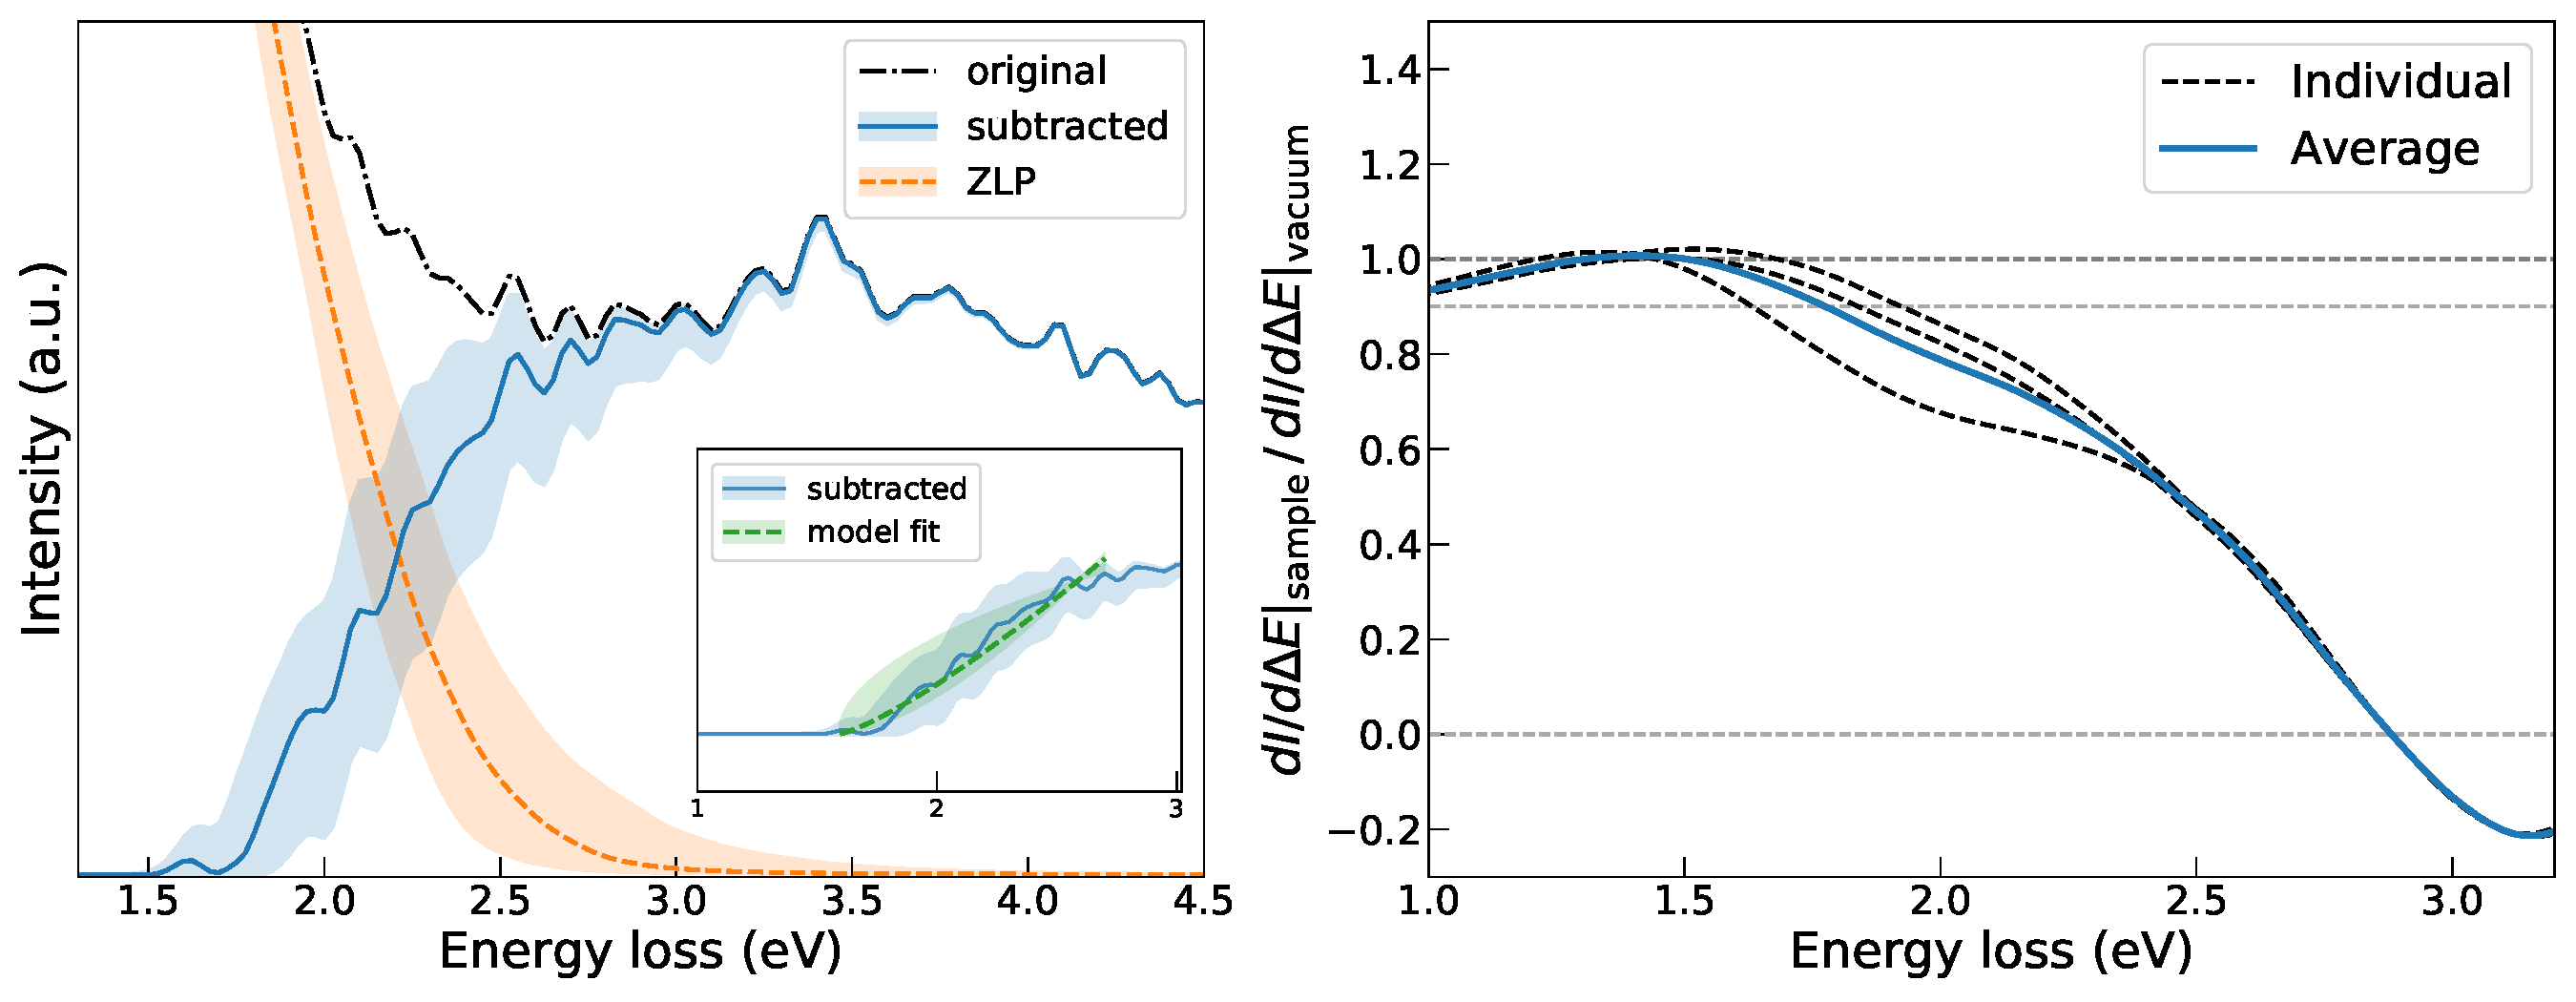
\includegraphics[width=0.99\linewidth]{plots/SubtractedEELS_plot_sp14.pdf}
   \caption{Left: the original
     and subtracted EEL spectra corresponding to location sp4 of sample A in Fig.~\ref{fig:ws2positions},
     together with the predictions of the ZLP model, where
     the bands indicate the 68\% confidence level uncertainties.
     %
     The inset displays the result of fitting Eq.~(\ref{eq:I1}) to the onset
     region of the subtracted spectrum.
     %
     Right: the average ratio of the derivative of the intensity
     distribution in sp4 over its vacuum counterparts, Eq.~(\ref{eq:rder})
  }
\label{fig:sp14_subtracted_spectrum}
\end{centering}
\end{figure}
%%%%%%%%%%%%%%%%%%%%%%%%%%%%%%%%%%%%%%%%%%%%%%%%%%%%%%%%%%%%%%%%%%%%%%%%%%

One can observe how the ZLP model uncertainties are small at low $\Delta E$
(due to the matching condition) and large $\Delta E$ (where the ZLP vanishes),
but become significant in the intermediate region where the contributions
from $I_{\rm ZLP}$ and $I_{\rm inel}$ become comparable.
%
It is worth emphasizing that these (unavoidable) uncertainties are neglected in most
ZLP subtraction methods.
%
The validity of our choice for the hyperparameter $\Delta E_{\rm I}$ (Table~\ref{table:sampledata_summary})
can be verified {\it a posteriori} by evaluating the ratio
\be
\mathcal{R}^{(j)}_{\rm abs}\lp \Delta E_{\rm I}\rp \equiv 
\la I_{\rm ZLP}^{({\rm mod})(j)}\ra_{\rm rep} \Big/I_{\rm EEL}^{({\rm exp})(j)} \Big|_{\Delta E = \Delta E_{\rm I}} \, ,
\ee
which in this case turns out to be $\mathcal{R}_{\rm abs} = 0.98$.
%
It is indeed important to verify that $\mathcal{R}_{\rm abs}\lp \Delta E_{\rm I}\rp$ is not too far from unity,
indicating that the training dataset has not been contaminated by the  contributions
arising from inelastic scatterings off the specimen.

The average ratio of the derivative of the intensity
distribution in sp4 over its vacuum counterpart, Eq.~(\ref{eq:rder}), is shown
in the right panel of  Fig.~\ref{fig:sp14_subtracted_spectrum}. 
%
By requiring that $\mathcal{R}_{\rm der}(\Delta E_{\rm I})\simeq 0.9$ we obtain
the value $\Delta E_{\rm I}=1.8$ eV used as baseline in the analysis.
%
It should be noted that this choice is not unique, for example requiring
$\mathcal{R}_{\rm der}(\Delta E_{\rm I})\simeq 0.8$ instead would have led
to $\Delta E_{\rm I}=2.0$ eV.
%
It is therefore important to asses the stability of our results as the hyper-parameter $\Delta E_{\rm I}$
is varied around its optimal value.
%
With this motivation, in Fig.~\ref{fig:bvalues_sampleA} we display the
values of the exponent $b$
and the bandgap energy $E_{\rm BG}$ 
obtained from the same subtracted spectrum as that shown in
Fig.~\ref{fig:sp14_subtracted_spectrum} for variations of $\Delta E_{\rm I}$ 
around its optimal value (vertical dot-dashed line) by an amount
of $\pm 0.2$ eV.
%
We observe that the model predictions for both $b$ and $E_{\rm BG}$ are stable with respect
to variations of $\Delta E_{\rm I}$, with shifts in central values contained within the
uncertainty bands.
%
We can thus conclude that our approach is robust with respect to the choice of
hyper-parameters.

%%%%%%%%%%%%%%%%%%%%%%%%%%%%%%%%%%%%%%%%%%%%%%%%%%%%%%%%%%
\begin{figure}[t]
\begin{centering}
  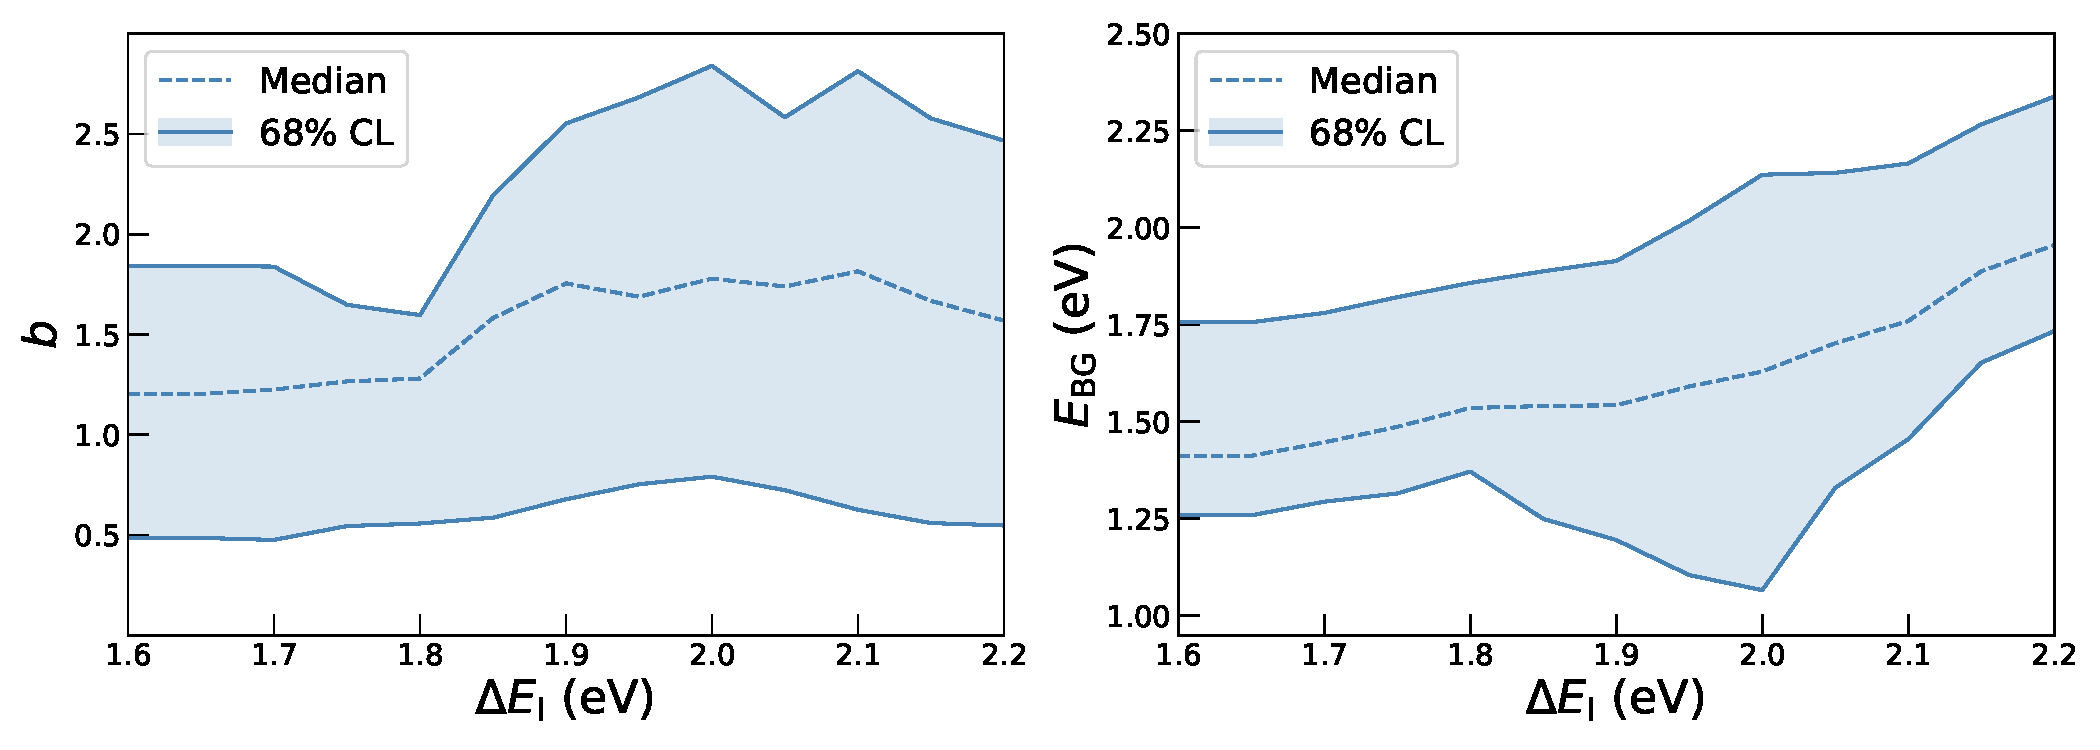
\includegraphics[width=0.99\linewidth]{plots/Stability_plots_sp14.pdf} 
  \caption{\small The values of the exponent $b$ (left)
    and the bandgap energy $E_{\rm BG}$ (right panel) from the model Eq.~(\ref{eq:I1})
    obtained from the subtracted spectrum sp14 as $\Delta E_{\rm I}$ is varied by $\pm 0.2$ eV
    around its optimal value, indicated by the horizontal dot-dashed line.
  }
\label{fig:bvalues_sampleA}
\end{centering}
\end{figure}
%%%%%%%%%%%%%%%%%%%%%%%%%%%%%%%%%%%%%%%%%%%%%%%%%%%%%%%%%%%%%

The final values for $E_{\rm BG}$ and $b$ obtained in the analysis of this specific spectrum are
\be
E_{\rm BG} = 1.6_{-0.2}^{+0.3}\,{\rm eV} \, ,\quad b= 1.3_{-0.7}^{+0.3} \, .
\ee
We thus find that for this specific region of the WS$_2$ nanoflowers
the model fit to the subtracted EEL spectrum exhibits a clear preference
for an indirect bandgap (where $b\simeq 1.5$ is expected).
%
This result is consistent with previous studies of the local
electronic properties of bulk WS$_2$, such as those reported in Table~\ref{table:bgvalues}.
%
Consistent results are obtained for spectra acquired at
other locations of Fig.~\ref{fig:ws2positions}; for example for sp5 one has
\be
E_{\rm BG} = 1.7 \pm 0.2\,{\rm eV} \, ,\quad b= 1.3_{-0.4}^{+0.3} \, .
\ee
%
These results represent the first EELS-based bandgap determination of WS$_2$ nanostructures
whose crystalline structure is based on mixed 2H/3R polytypes.

\subsection{Mapping excitonic transitions in the low-loss region}

For the application of our ZLP subtraction strategy to the EEL spectra recorded in specimen B
of the WS$_2$ nanoflowers (bottom panels
in  Fig.~\ref{fig:ws2positions}), the same criterion
based on the derivative ratio Eq.~(\ref{eq:rder}) to select the hyper-parameter $\Delta E_{\rm I}$ was
used.
%
In this case, one finds a value of $\Delta E_{\rm I}\simeq 1.4$ eV,
 somewhat lower than the corresponding value obtained for sample A.
%
The left panel of Fig.~\ref{fig:SubtractedEELS_plot_sp4} displays
the original
and subtracted spectra corresponding to the representative
location sp4 of sample B
together with the predictions of the ZLP model.
%
As before, the bands indicate the 68\% confidence level uncertainties
and the central value is the median.

The main difference with respect to the spectra recorded in sample A is the appearance
of well-defined features (peaks) in the subtracted spectrum already for
very small values of $\Delta E$.
%
In particular, we observe two marked peaks at $\Delta E\simeq 1.5$ and 2.0 eV and a
softer one near $\Delta E \simeq 1.7$ eV.
%
Further additional features arise also for higher values of the energy loss.
%
There are two main sources for the observed differences between the spectra recorded
in each sample.
%
The first one is that, while sample A is much thicker (bulk material), sample B corresponds
to thin, overlapping petals whose thicknesses can be as small as a few monolayers.
%
The second is that the EELS measurements taken in sample A used a TEM without monochromator,
while those in sample B benefited from a monochromator thus achieving a
superior
spectral resolution (with an average FWHM of 87 meV to be compared with the 470 meV of sample A, see
Table~\ref{table:sampledata}).
%
This combination of structural and morphological variations in the specimen together
with the operation conditions of the TEM therefore should account for the
most of differences
between the two sets of spectra.


%%%%%%%%%%%%%%%%%%%%%%%%%%%%%%%%%%%%%%%%%%%%%%%%%%%%%%%%%%%%%%%%%%%%%%%
\begin{figure}[t]
\begin{centering}
  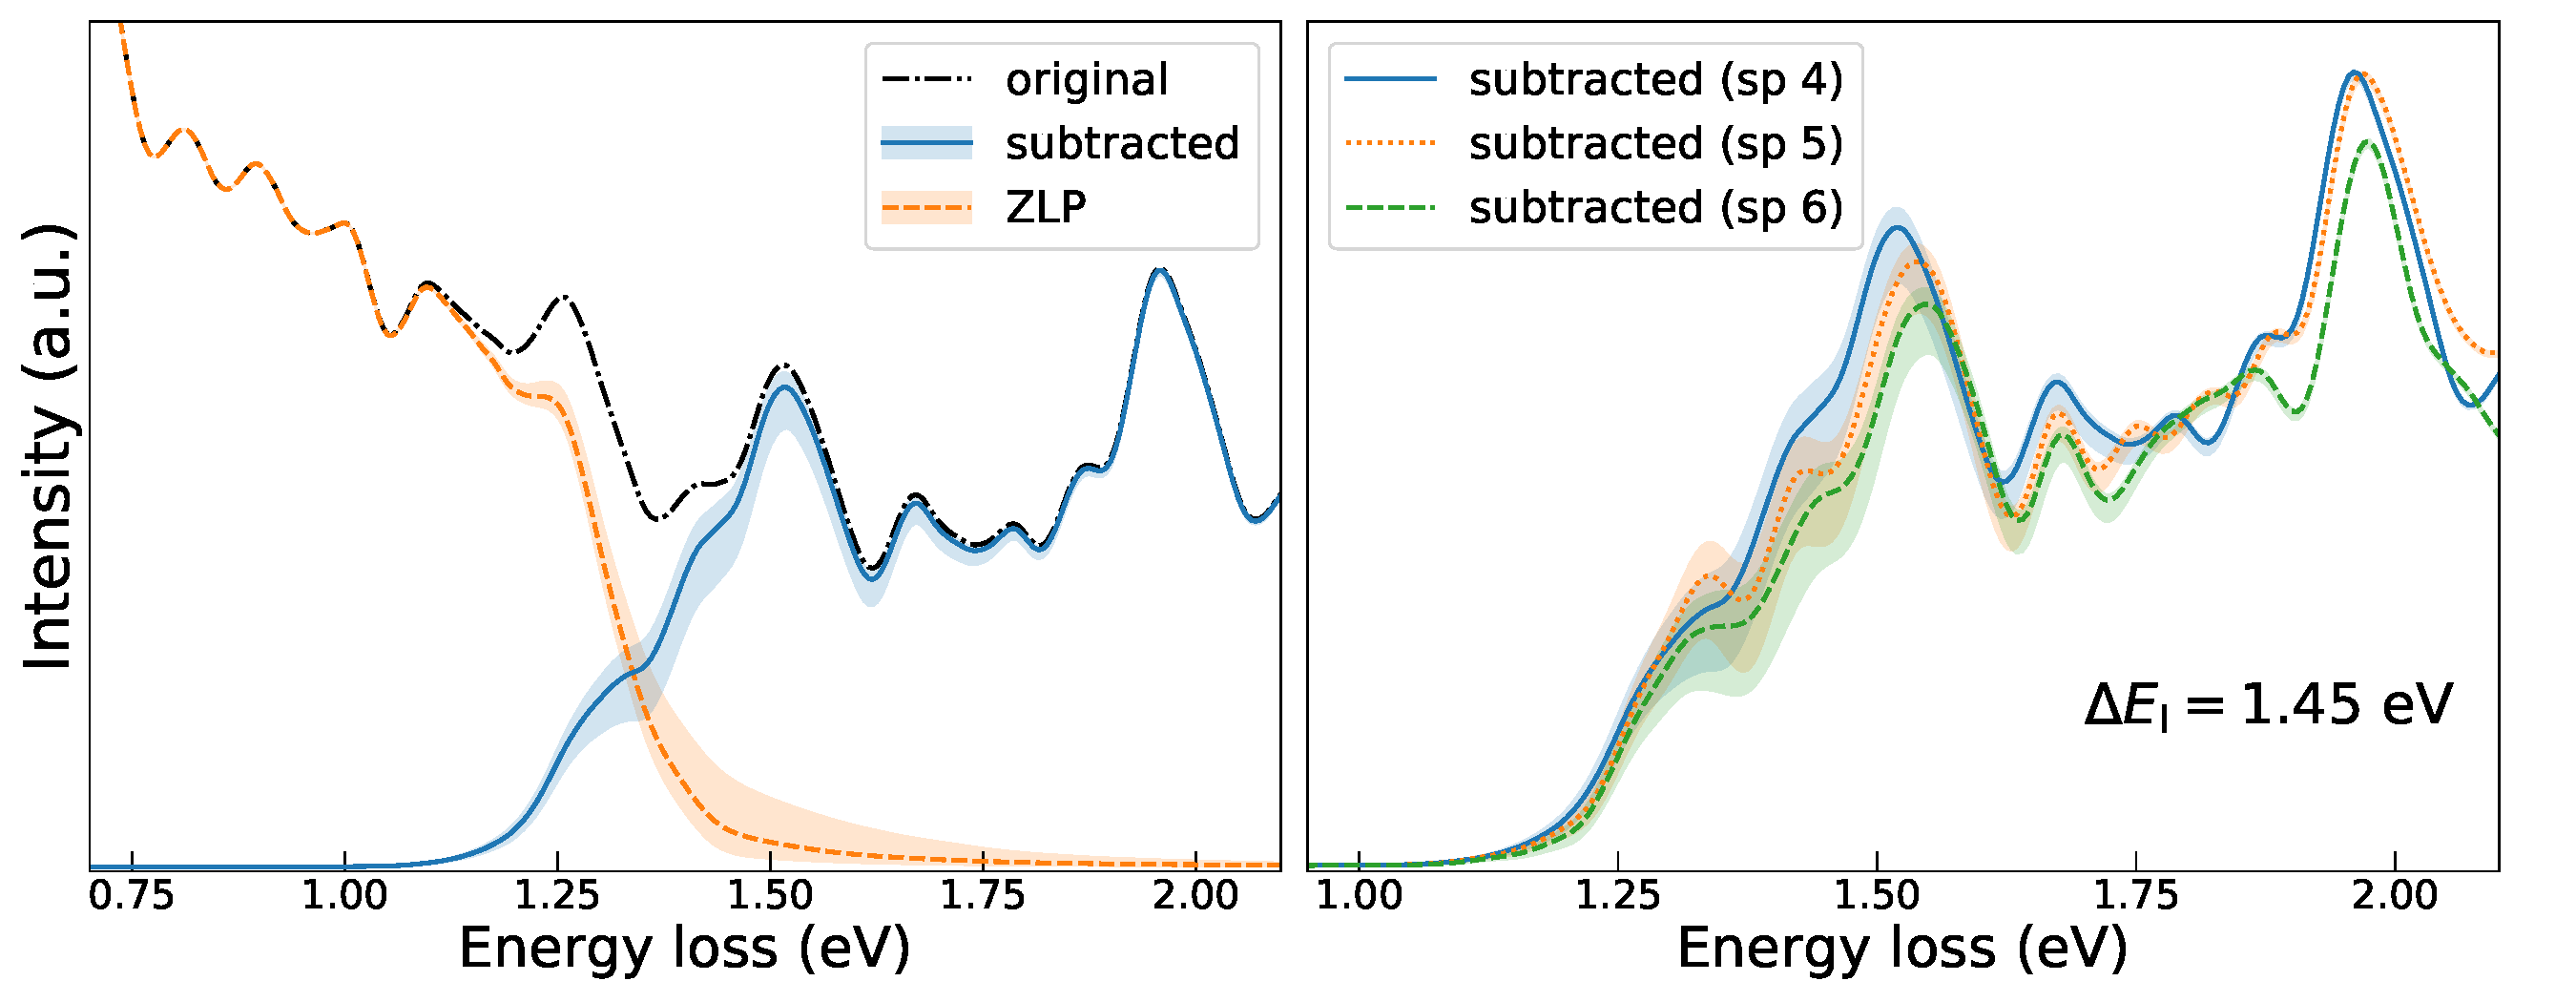
\includegraphics[width=0.99\linewidth]{plots/subtractedEELS_plot_sampleB_sp4.pdf}
  \caption{Left: the original
     and subtracted EEL spectra corresponding to location sp4 of sample B in Fig.~\ref{fig:ws2positions},
     together with the predictions of the ZLP model.
     %
     The bands indicate the 68\% confidence level uncertainties.
     %
     Right: comparison of the ZLP-subtracted spectra from locations sp4, sp5, and sp6 in sample B
     together with the corresponding model uncertainties.
    %
     Note how several features of the subtracted spectra, in particular
     the peaks at $\Delta E\simeq 1.5$,
    1.7 and 2.0 are eV, are common across the three locations.
  }
\label{fig:SubtractedEELS_plot_sp4}
\end{centering}
\end{figure}
%%%%%%%%%%%%%%%%%%%%%%%%%%%%%%%%%%%%%%%%%%%%%%%%%%%%%%%%%%%%%%%%%%%%%%%%%%


It is worth noting here that our ZLP parametrisation and subtraction strategy exhibits a satisfactory
performance for all the spectra under consideration, irrespective of the spectral resolution of the TEM used
for their acquisition.
%
By comparing Figs.~\ref{fig:SubtractedEELS_plot_sp4} and~\ref{fig:sp14_subtracted_spectrum}, one observes
that  model uncertainties are larger in the latter case than in the former, as expected from the
superior 
spectral resolution of the EELS measurements taken on sample B.
%
Nevertheless, the same approach has been used in both cases without the need of any fine-tuning
or {\it ad hoc} adjustments: of course, if the input
spectra have been recorded with better spectral resolution, the resulting ZLP model uncertainties
will improve accordingly without changing the procedure itself.

Given that the
well-defined spectral features present in Fig.~\ref{fig:SubtractedEELS_plot_sp4}
appear close to the onset of the inelastic emissions, $I_{\rm inel}(\Delta E)$,
these spectra are not suitable for bandgap determination analyses.
%
The reason is that the method of~\cite{Rafferty:2000}
used in sample A is only applicable under the assumption that there is a sufficiently wide region in $\Delta E$
after the onset of $I_{\rm inel}$ to perform the polynomial fit of Eq.~(\ref{eq:I1}).
%
This is clearly not possible  for the spectra recorded in sample B, and indeed model fits restricted to $\Delta E\le 1.4$ eV
display a marked numerical instability.
%
Instead of studying the bandgap properties, it is interesting to exploit the ZLP-subtracted results of sample B
to characterise the local
excitonic transitions of polytypic 2H/3R WS$_2$
that are known to arise in the ultra-low-loss region of the spectra.

Before being able to do this, however, one has to deal with the possible objection
that the peaks present in Fig.~\ref{fig:SubtractedEELS_plot_sp4} are not
genuine features, but rather fluctuations due to insufficient statistics
that should be smoothed out before this region can be interpreted.
%
To tackle this concern, the right panel of Fig.~\ref{fig:SubtractedEELS_plot_sp4}
displays a
comparison of the ZLP-subtracted spectra recorded in the (spatially separated) locations sp4, sp5 and sp6
in sample B
together with their model uncertainties.
%
Both the position and the widths of the peaks at $\Delta E\simeq 1.5$,
1.7 and 2.0 eV remain stable, confirming that these
are genuine physical features rather than fluctuations.

These peaks in the ultra-low-loss region of the ZLP-subtracted EELS spectra recorded on thin, polytypic
WS$_2$ nanostructures can be traced back to excitonic transitions.
%
Their origin can be attributed to the formation of an electron-hole pair mitigated
by the dielectric screening from the surrounding lattice~\cite{Hanbicki:2016}.
%
In nanostructures with reduced dimensionality as well as in single layers of TMD materials,
exciton peaks arise with binding energies up to ten times larger than for bulk structures.
%
In the optical spectra of TMDs, two strongly pronounced resonances denoted by A and B
excitons are often observed, appearing at binding energies of 300 and
500 meV below the true band gap of the material~\cite{Karivaj:2019}.
%
Interestingly, this prediction is in agreement with the observed peaks at
$\Delta E\simeq 1.5$ and 1.7 eV if one takes into account the expected
value of $E_{\rm BG}$ for very thin  WS$_2$ nanostructures, see Table~\ref{table:bgvalues}

We  conclude that ZLP-subtracted spectra in sample B allow one for
a clean mapping of the exciton peaks present in the WS$_2$ nanoflowers
down to $\Delta E\simeq 1.5$ eV together with
the associated uncertainty estimate.
%
Further insights concerning the relationship between the exciton peaks in the ultra-low-loss region
and the underlying crystalline structure and specimen morphology could be obtained
by combining our findings with {\it ab initio} calculations such as those based on
density functional theory.
